%%%%%%%%%%%%%%%%%%%%%%%%%%%%%%%%%%%%%%%% Pakete
\documentclass[10pt,a4paper]{article}

%Schrift-Packages
\usepackage[ngerman]{babel}		%% neue deutsche Rechtschreibung
\usepackage[utf8x]{inputenc}    %% fügt Umlaute hinzu
\PrerenderUnicode{ä}            %% für Umlaute auf der Titelseite 
\PrerenderUnicode{ö}
\PrerenderUnicode{ü}
\PrerenderUnicode{ß}
\usepackage[T1]{fontenc}        %% for selecting font encodings
\usepackage{lmodern}            %% besseres Schriftbild für PDFs
\usepackage{ucs}                %% extended UTF-8 input encoding support

\usepackage{amssymb}            %% extended math symbol collection
\usepackage{amsmath}            %% miscellaneous enhancements for formulas   
\usepackage{graphicx}           %% für das Einfügen von Bildern
\usepackage{pdfpages}           %% für das Einbinden von PDFs



\usepackage{geometry}           %% Gestaltung einer Seite
\geometry{a4paper}              %% Voreinstellung für A4-Seiten

\usepackage{booktabs}           %% enhances the quality of tables
\usepackage{float}              %% Improves the interface for defining floating objects such as figures and tables
\usepackage[absolute]{textpos}  %% facilitate placement of boxes at absolute positions
\usepackage{ulem}               %% Unterstreichen von Absätzen

\usepackage[skins]{tcolorbox}   %% environment for coloured and framed text boxes

\usepackage{subfigure}          %% manipulation and reference of small or 'sub' figures and tables 

\usepackage{titling}            %% control over the typesetting of the \maketitle command and \thanks commands

\usepackage{fancyhdr}           %% control of page headers and footers

\definecolor{fh_green}{RGB}{121,167,24}     %% FH-Farben werden hier definiert
\definecolor{fh_grey}{RGB}{95,100,103}
\definecolor{fh_blue}{RGB}{10,79,138} 

\pagestyle{fancy}               
\fancyhead[R]{\leftmark}        %% Voreinstellung der Kopfzeile
%%%%%%%%%%%%%%%%%%%%%%%%%%%%%%%%%%%
%%%%%%%%%%%%%%%%%%%%%%%%%%%%%%%%%%%
%%%%%%%%%%%%%%%%%%%%%%%%%%%%%%%%%%% 

%%% Hier Kapitel, Titel, AutorInnen, Studiengang, Lehrveranstaltung, BetreuerIn und Erstellungsdatum angeben: %%%

\newcommand{\thema}{Laborprotokoll}
\title{Titel des Versuchs}
\author{Vorname Nachname, Vorname Nachname}
\newcommand{\studiengang}{Studiengang}
\newcommand{\lehrveranstaltung}{Lehrveranstaltung}
\newcommand{\betreuerin}{Max Mustermann}
\newcommand{\erstellungsdatum}{1.1.1994}


%%%%%%%%%%%%%%%%%%%%%%%%%%%%%%%%%%%
%%%%%%%%%%%%%%%%%%%%%%%%%%%%%%%%%%%
%%%%%%%%%%%%%%%%%%%%%%%%%%%%%%%%%%% Doument (Anfang)
\begin{document}
%%%%%%%%%%%%%%%%%%%%%%%%%%%%%%%%%%%
%%%%%%%%%%%%%%%%%%%%%%%%%%%%%%%%%%%
%%%%%%%%%%%%%%%%%%%%%%%%%%%%%%%%%%% Titelseite (Anfang)
\begin{titlepage}

\begin{textblock}{3}(-0.4,0)

\includegraphics{bilder/Deckblatt.pdf}
\end{textblock}
%Titel
\mbox{}

\begin{textblock}{8}(2,3)

\noindent \Huge \textbf{\thema}

\noindent \Huge  \thetitle
\end{textblock}

%Author & Datum
\begin{textblock}{12.5}(1.5,11.5)

\Large Erstellt von: \hfill \theauthor

\Large Studiengang: \hfill \studiengang

\Large Lehrveranstaltung: \hfill \lehrveranstaltung

\Large BetreuerIn: \hfill \betreuerin

\Large Wien, am \erstellungsdatum 
\end{textblock}
\end{titlepage}
%%%%%%%%%%%%%%%%%%%%%%%%%%%%%%%%%%%
%%%%%%%%%%%%%%%%%%%%%%%%%%%%%%%%%%%
%%%%%%%%%%%%%%%%%%%%%%%%%%%%%%%%%%% Titelseite (Ende)
\newpage
%%%%%%%%%%%%%%%%%%%%%%%%%%%%%%%%%%% Inhaltsverzeichnis (Anfang)
\thispagestyle{plain}
\tableofcontents
%%%%ö%%%%%%%%%%%%%%%%%%%%%%%%%%%%%% Inhaltsverzeichnis (Ende)
\newpage
%%%%%%%%%%%%%%%%%%%%%%%%%%%%%%%%%%% Inhalt (Anfang)

\section{Einleitung}

Die Motivation, Fragestellung und Inhalt des Experiments erläutert.

\subsection{Theorie}

Benötigte theoretische Grundlagen und Formeln
\begin{equation}
\bar{x} = \frac{x_1 + x_2 + ... + x_N}{N} = \frac{1}{N} \sum_{i=1}^N x_{i}
\label{Mittelwert}
\end{equation}
werden erläutert und gegebenenfalls auf Quellen verwiesen \cite{balzert}. 

%%%%%%%%%%%%%%%%%%%%%%%%%%%%%%%%%%%

\section{Durchführung} %Bei komplexeren Versuchen können Sie Versuchsaufbau, Methodik und Durchführung auch als seperate Kapitel oder mittels \subsection als Unterkapitel behandeln.

Der Versuchsaufbau, die Methodik und das Vorgehen werden erklärt. 

\begin{figure}[H]
\centering
    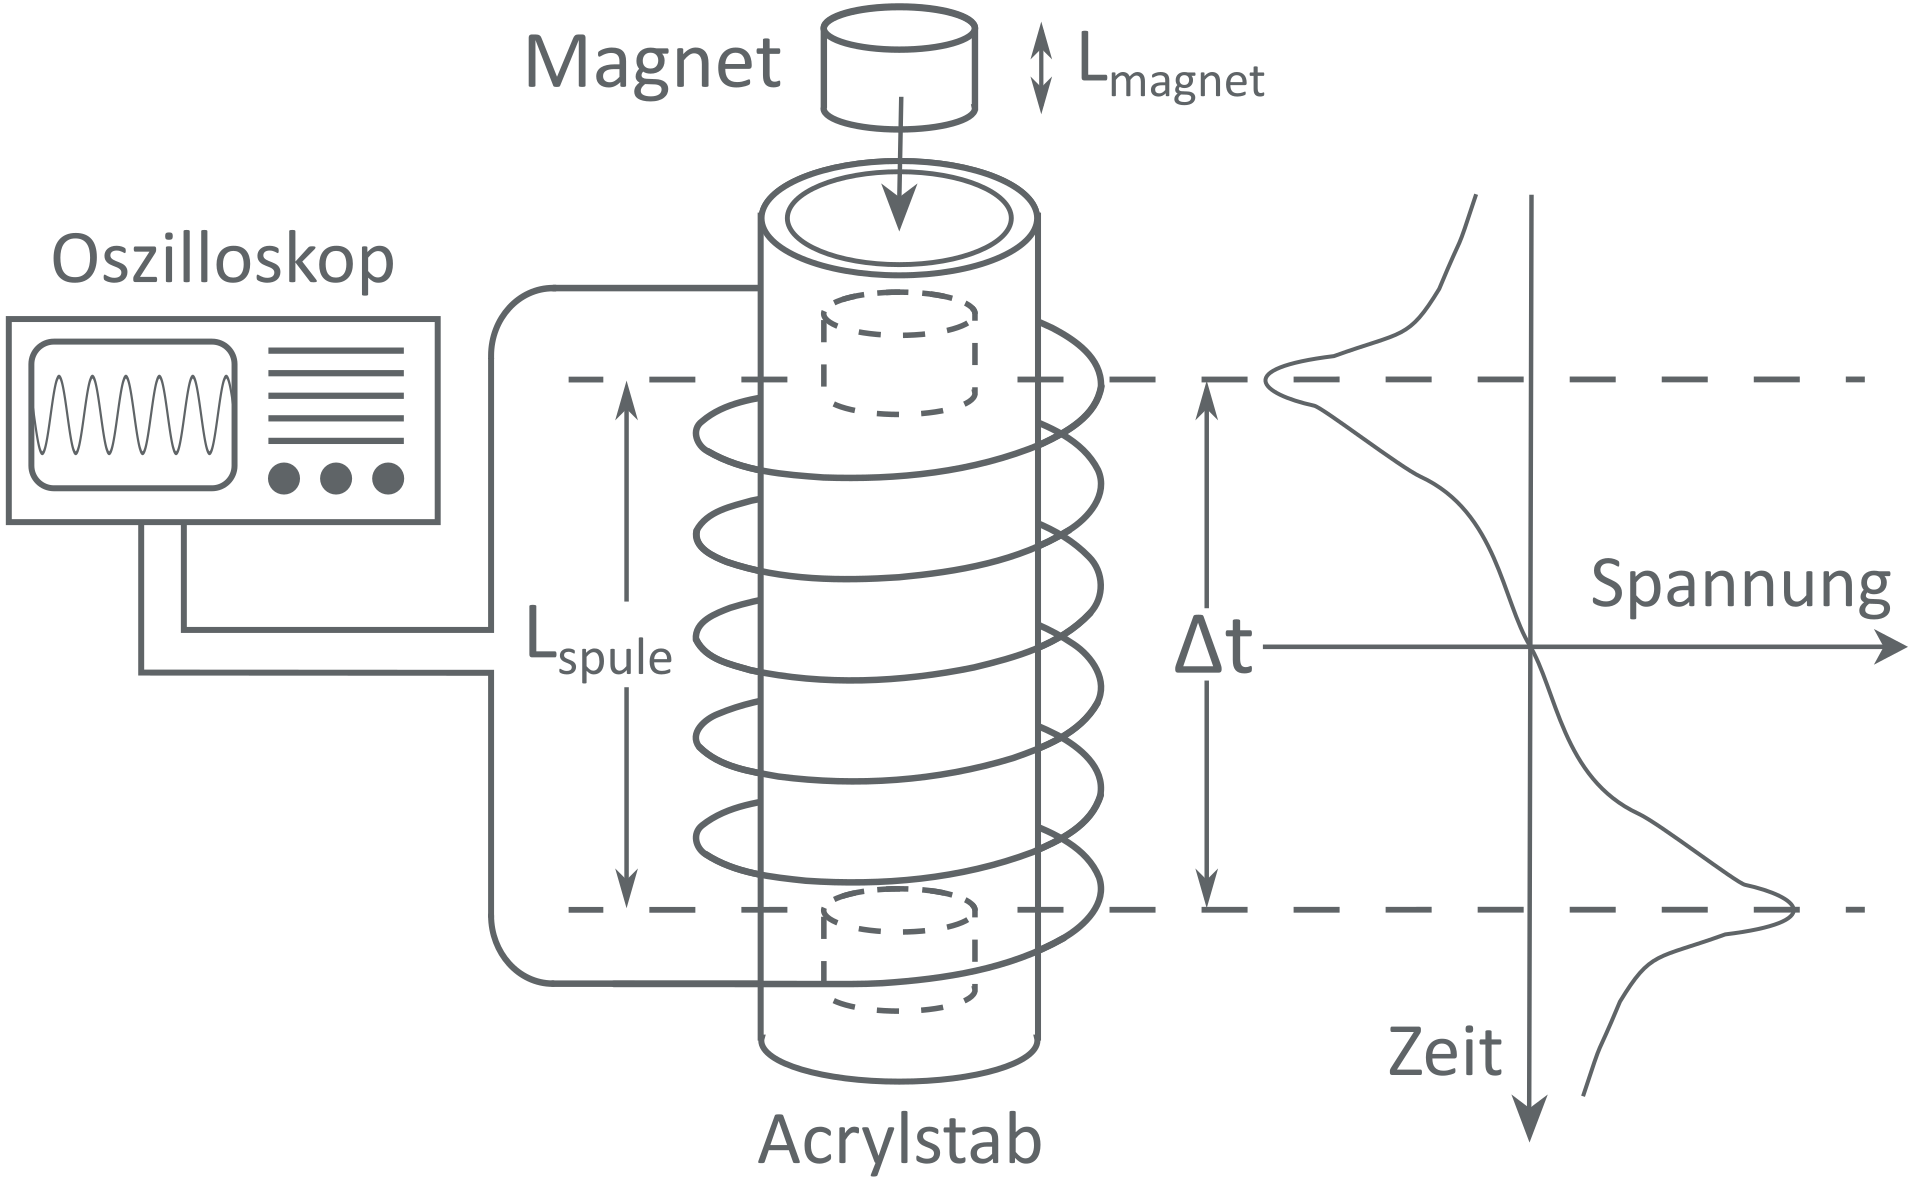
\includegraphics[scale=0.25]{bilder/Aufbau.png}
  \caption{Skizze eines Versuchsaufbaus \cite{ind}}
  \label{Versuchsaufbau}
\end{figure}

Die Rohdaten werden gezeigt oder darauf verwiesen, wo sie zu finden sind (siehe Anhang A).

\begin{table}[H]
\center
\begin{tabular}{crrr}
\toprule
Messung & x [m] & t [s] & v [m/s] \\
\midrule
1 & 0.2 & 0.20 & 1.98 \\
2 & 0.4 & 0.29 & 2.80 \\
3 & 0.6 & 0.35 & 3.43 \\
4 & 0.8 & 0.40 & 3.96 \\
5 & 1.0 & 0.45 & 4.43 \\
\bottomrule
\end{tabular}
\caption{Sie können https://www.tablesgenerator.com/ zur einfacheren Formatierung von Tabellen verwenden.}
\label{tabelle1}
\end{table}

%%%%%%%%%%%%%%%%%%%%%%%%%%%%%%%%%%%%%%%%

\section{Auswertung und Diskussion} %Auch hier können bei ausführlichen Auswertungen und Diskussionen die Kapitel getrennt werden.

Die Messwerte werden verarbeitet, unbekannte Größen und deren Fehler berechnet und analysiert, die Endergebnisse dargestellt und diskutiert, auf Fragestellungen eingegangen.

\medskip

\centerline{$x = (\bar{x} \pm \sigma_x) [Einheit]$}

\medskip

\centerline{\colorbox{fh_green}{$y = (\bar{y} \pm \sigma_y) [Einheit]$}}

\medskip

\centerline{\fbox{\colorbox{fh_green}{$z = (\bar{z} \pm \sigma_z) [Einheit]$}}}

\begin{figure}[H]
\centering
    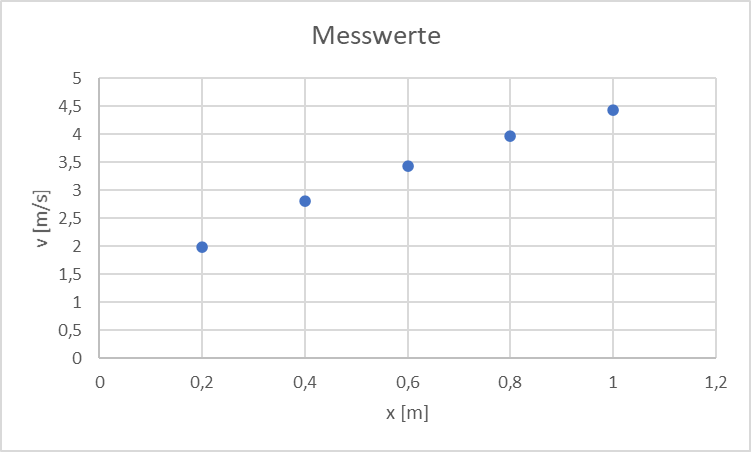
\includegraphics[scale=2]{bilder/Messwerte.png}
  \caption{Graphische Darstellung der Ergebnisse}
  \label{Ergebnisse}
\end{figure}

%%%%%%%%%%%%%%%%%%%%%%%%%%%%%%%%%%%
%%%%%%%%%%%%%%%%%%%%%%%%%%%%%%%%%%%
%%%%%%%%%%%%%%%%%%%%%%%%%%%%%%%%%%% Hier ist die verwendete Literatur anzugeben, auf die sie mit \cite{Name} verweisen können.

\newpage

\addcontentsline{toc}{section}{Literatur} 
\begin{thebibliography}{-----}

\bibitem[1]{balzert}H. Balzert, \textit{Lehrbuch der Objektmodellierung - Analyse und Entwurf mit der UML 2}, 2. Ausg., Elsevier GmbH, München 2005.

\bibitem[2]{ind} J. Schmid, G. Krizek: \textit{Versuche zur Induktion einer Spannung in einer Spule}; Laboranleitung der FH Technikum Wien;

\end{thebibliography}

%%%%%%%%%%%%%%%%%%%%%%%%%%%%%%%%%%%
%%%%%%%%%%%%%%%%%%%%%%%%%%%%%%%%%%%
%%%%%%%%%%%%%%%%%%%%%%%%%%%%%%%%%%%

\newpage

\appendix

\section{Anhang}

\begin{table}[H]
\center
\begin{tabular}{crrr}
\toprule
Messung & x [m] & t [s] & v [m/s] \\
\midrule
1 & 0.2 & 0.20 & 1.98 \\
2 & 0.4 & 0.29 & 2.80 \\
3 & 0.6 & 0.35 & 3.43 \\
4 & 0.8 & 0.40 & 3.96 \\
5 & 1.0 & 0.45 & 4.43 \\
\bottomrule
\end{tabular}
\caption{Messwerte Anhang}
\label{tabelleanhang}
\end{table}

\begin{figure}[H]
\centering
    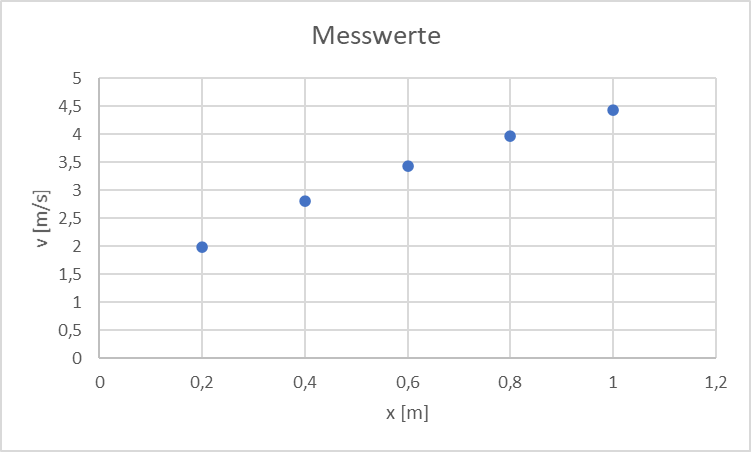
\includegraphics[scale=2]{bilder/Messwerte.png}
  \caption{Grafik Anhang}
  \label{grafikanhang}
\end{figure}

%%%%%%%%%%%%%%%%%%%%%%%%%%%%%%%%%%% Inhalt (Ende)
\end{document}
%%%%%%%%%%%%%%%%%%%%%%%%%%%%%%%%%%% Dokument (Ende)
